\documentclass[12pt]{report}
\usepackage[utf8]{inputenc}
\usepackage[russian]{babel}
%\usepackage[14pt]{extsizes}
\usepackage{listings}
\usepackage{graphicx}
\usepackage{amsmath,amsfonts,amssymb,amsthm,mathtools} 
\usepackage{pgfplots}
\usepackage{filecontents}
\usepackage{float}
\usepackage{comment}
\usepackage{indentfirst}
\usepackage{eucal}
\usepackage{enumitem}
%s\documentclass[openany]{book}
\frenchspacing

\usepackage{indentfirst} % Красная строка

\usetikzlibrary{datavisualization}
\usetikzlibrary{datavisualization.formats.functions}

\usepackage{amsmath}


% Для листинга кода:
\lstset{ %
	language=c,                 % выбор языка для подсветки (здесь это С)
	basicstyle=\small\sffamily, % размер и начертание шрифта для подсветки кода
	numbers=left,               % где поставить нумерацию строк (слева\справа)
	numberstyle=\tiny,           % размер шрифта для номеров строк
	stepnumber=1,                   % размер шага между двумя номерами строк
	numbersep=5pt,                % как далеко отстоят номера строк от подсвечиваемого кода
	showspaces=false,            % показывать или нет пробелы специальными отступами
	showstringspaces=false,      % показывать или нет пробелы в строках
	showtabs=false,             % показывать или нет табуляцию в строках
	frame=single,              % рисовать рамку вокруг кода
	tabsize=2,                 % размер табуляции по умолчанию равен 2 пробелам
	captionpos=t,              % позиция заголовка вверху [t] или внизу [b] 
	breaklines=true,           % автоматически переносить строки (да\нет)
	breakatwhitespace=false, % переносить строки только если есть пробел
	escapeinside={\#*}{*)}   % если нужно добавить комментарии в коде
}


\usepackage[left=2cm,right=2cm, top=2cm,bottom=2cm,bindingoffset=0cm]{geometry}
% Для измененных титулов глав:
\usepackage{titlesec, blindtext, color} % подключаем нужные пакеты
\definecolor{gray75}{gray}{0.75} % определяем цвет
\newcommand{\hsp}{\hspace{20pt}} % длина линии в 20pt
% titleformat определяет стиль
\titleformat{\chapter}[hang]{\Huge\bfseries}{\thechapter\hsp\textcolor{gray75}{|}\hsp}{0pt}{\Huge\bfseries}


% plot
\usepackage{pgfplots}
\usepackage{filecontents}
\usetikzlibrary{datavisualization}
\usetikzlibrary{datavisualization.formats.functions}

\begin{document}
	%\def\chaptername{} % убирает "Глава"
	\thispagestyle{empty}
	\begin{titlepage}
		\noindent \begin{minipage}{0.15\textwidth}
			
\includegraphics[width=\linewidth]{img/b_logo}
		\end{minipage}
		\noindent\begin{minipage}{0.9\textwidth}\centering
			\textbf{Министерство науки и высшего образования Российской Федерации}\\
			\textbf{Федеральное государственное бюджетное образовательное учреждение высшего образования}\\
			\textbf{~~~«Московский государственный технический университет имени Н.Э.~Баумана}\\
			\textbf{(национальный исследовательский университет)»}\\
			\textbf{(МГТУ им. Н.Э.~Баумана)}
		\end{minipage}
		
		\noindent\rule{18cm}{3pt}
		\newline\newline
		\noindent ФАКУЛЬТЕТ $\underline{\text{«Информатика и системы управления»}}$ \newline\newline
		\noindent КАФЕДРА $\underline{\text{«Программное обеспечение ЭВМ и информационные технологии»}}$\newline\newline\newline\newline\newline
		
		\begin{center}
			\noindent\begin{minipage}{1.1\textwidth}\centering
				\Large\textbf{  Отчет по лабораторной работе №1}\newline
				\textbf{по дисциплине <<Математическая статистика>>}\newline\newline\newline
			\end{minipage}
		\end{center}
		
		\noindent\textbf{Тема} $\underline{\text{Гистрограмма и эмпирическая функция распределения}}$\newline\newline
		\noindent\textbf{Студент} $\underline{\text{Нгуен Фыок Санг~~~~~~~~~~~~~~~~~~~~~~~~~~~~~~~~~~~~~~~~~~~~~~~~~~~~~}}$\newline\newline
		\noindent\textbf{Группа} $\underline{\text{ИУ7-66Б~~~~~~~~~~~~~~~~~~~~~~~~~~~~~~~~~~~~~~~~~~~~~~~~~~~~~~~~~~~~~}}$\newline\newline
		\noindent\textbf{Оценка (баллы)} $\underline{\text{~~~~~~~~~~~~~~~~~~~~~~~~~~~~~~~~~~~~~~~~~~~~~~~~~~~~~~~~~~~~}}$\newline\newline
		\noindent\textbf{Преподаватель} $\underline{\text{Саркисян П. С.~~~~~~~~~~~~~~~~~~~~~~~~~~~~~~~~~~~~~~~~~}}$\newline\newline\newline
		
		\begin{center}
			\vfill
			Москва~---~\the\year
			~г.
		\end{center}
	\end{titlepage}

\chapter*{Задание}

\section*{Цель работы}
Построение гистограммы и эмпирической функции распределения.

\section*{Постановка задачи}

\begin{enumerate}
	\item Для выборки объёма $n$ из генеральной совокупности $X$ реализовать в виде программы на ЭВМ
	\begin{enumerate}
		\item вычисление максимального значения $M_{\max}$ и минимального значения $M_{\min}$;
		\item размаха $R$ выборки;
		\item вычисление оценок $\hat\mu$ и $S^2$ математического ожидания $MX$ и дисперсии $DX$;
		\item группировку значений выборки в $m = [\log_2 n] + 2$ интервала;
		\item построение на одной координатной плоскости гистограммы и графика функции плотности распределения вероятностей нормальной случайной величины с математическим ожиданием $\hat{\mu}$ и дисперсией $S^2$;
		\item построение на другой координатной плоскости графика эмпирической функции распределения и функции распределения нормальной случайной величины с математическим ожиданием $\hat{\mu}$ и дисперсией $S^2$.
	\end{enumerate}
	\item Провести вычисления и построить графики для выборки из индивидуального варианта.
\end{enumerate}

\chapter*{Теоретические сведения}

\section*{Формулы для вычисления величин}

\subsection*{Минимальное и максимальное значения выборки}
\begin{equation}
	\begin{aligned}
	M_{\max} = X_{(n)}\\
	M_{\min} = X_{(1)}
	\end{aligned}
\end{equation}

\subsection*{Размах выборки}
\begin{equation}
	R = M_{\max} - M_{\min}.
\end{equation}

\subsection*{Оценки математического ожидания и дисперсии}
\begin{equation}
	\begin{aligned}
	\hat\mu(\vec X_n) &= \frac 1n \sum_{i=1}^n X_i\\
	S^2(\vec X_n) &= \frac 1{n-1} \sum_{i=1}^n (X_i-\overline X_n)^2
	\end{aligned}
\end{equation}

\section*{Определение эмпирической плотности и гистограммы}

Пусть $\vec x$ -- выборка из генеральной совокупности $X$. Если объем $n$ этой выборки велик, то значения $x_i$ группируют в интервальный статистический ряд. Для этого отрезок $J = [x_{(1)}, x_{(n)}]$ делят на $m$ равновеликих частей:

\begin{equation*}
	J_i = [x_{(1)} + (i - 1) \cdot \Delta, x_{(1)} + i \cdot \Delta), i = \overline{1; m - 1}
\end{equation*}

\begin{equation*}
	J_{m} = [x_{(1)} + (m - 1) \cdot \Delta, x_{(n)}]
\end{equation*}

\begin{equation*}
	\Delta = \frac{|J|}{m} = \frac{x_{(n)} - x_{(1)}}{m}
\end{equation*}

Интервальным статистическим рядом называют таблицу:

\begin{table}[htb]
	\centering
	\begin{tabular}{|c|c|c|c|c|}
		\hline
		$J_1$ & ... & $J_i$ & ... & $J_m$ \\
		\hline
		$n_1$ & ... & $n_i$ & ... & $n_m$ \\
		\hline
	\end{tabular}
\end{table}

где $n_i$ -- количество элементов выборки $\vec x$, которые $\in J_i$.

Обычно выборку разбивают на $m=[\log_2n]+2$ интервалов, где $n$ -- размер выборки.

Гистограмма -- это график эмпирической плотности. 

\textit{Эмпирической плотностью}, отвечающей выборке $\vec x$, называют функцию:
\begin{equation}
	\hat f(x) =
	\begin{cases}
	\frac{n_i}{n \Delta}, x \in J_i, i = \overline{1; m} \\
	0, \text{иначе} \\
	\end{cases}
\end{equation}

где $J_i$ -- полуинтервал статистического ряда, $n_i$ -- количество элементов выборки, входящих в полуинтервал, $n$ -- количество элементов выборки.

\section*{Определение эмпирической функции распределения}

Пусть $\vec x = (x_1, ..., x_n)$ -- выборка из генеральной совокупности $X$. Обозначим $n(x, \vec x)$ -- число элементов вектора $\vec x$, которые имеют значения меньше $x$.

\textit{Эмпирической функцией распределения} называют функцию $F_n: \mathbb{R} \to \mathbb{R}$, определенную как: 

\begin{equation}
	F_n(x) = \frac{n(x, \vec x)}{n}
\end{equation}

\chapter*{Результаты работы программы}

\section*{Код программы}

\begin{lstlisting}[language=Matlab]

function lab1()
	clear all;
	X = [10.06,8.32,8.50,8.82,6.02,6.44,7.90,7.85,5.90,7.62,8.66,...
	6.38,7.24,8.21,6.82,7.43,6.06,8.21,9.07,5.85,6.72,8.17,...
	8.53,8.68,7.21,8.43,8.77,7.27,5.79,9.78,6.44,7.24,6.83,...
	6.61,7.58,10.15,8.82,7.87,7.35,9.60,5.82,6.65,10.15,6.92,...
	6.77,9.35,6.92,7.76,6.45,7.47,6.99,9.95,7.22,7.38,7.87,...
	6.24,8.00,8.47,7.25,7.03,7.45,6.75,7.37,7.98,9.58,8.91,...
	6.14,8.19,5.07,7.47,7.29,8.78,7.86,7.82,10.09,8.54,7.21,...
	8.57,6.67,9.82,9.26,9.69,8.39,8.26,7.44,6.58,8.45,7.49,...
	7.16,9.17,8.16,8.38,7.60,8.53,6.10,7.39,7.70,8.45,7.73,...
	9.21,8.02,7.62,6.90,9.55,5.73,7.21,6.14,7.54,9.87,8.14,...
	8.16,7.50,7.60,6.25,7.03,7.07,6.61,9.68,7.65,8.32];
	X = sort(X);
	
	Mmax = max(X);
	Mmin = min(X);
	
	fprintf('Mmin = %s\n', num2str(Mmin));
	fprintf('Mmax = %s\n', num2str(Mmax));
	
	R = Mmax - Mmin;
	fprintf('R = %s\n', num2str(R));
	
	MX = getMU(X);
	fprintf('MX = %s\n', num2str(MX));
	
	S2 = getS2(X);
	fprintf('S^2 = %s\n', num2str(S2));
	
	m = getNumberOfIntervals(X);
	fprintf('m = %s\n', num2str(m))
	
	
	createGroup(X);
	hold on;
	distributionDensity(X, MU, S2, m);
	
	figure;
	empiricF(X);
	hold on;
	distribution(X, MU, S2, m);
end

function mu = getMU(X)
	n = length(X);
	mu = sum(X)/n;
end

function S2 = getS2(X)
	n = length(X);
	MX = getMU(X);
	S2 = sum((X - MX).^2) / (n-1);
end

function m = getNumberOfIntervals(X)
	m = floor(log2(length(X)) + 2);
end

function createGroup(X)
	n = length(X);
	m = getNumberOfIntervals(X);
	
	intervals = zeros(1, m+1);
	numCount = zeros(1, m+1);
	
	MinX = min(X);
	Delta = (max(X) - min(X)) / m;
	fprintf('Delta = %s\n', num2str(Delta));
	
	for i = 0: m
	intervals(i+1) = MinX + Delta * i;
	end
	
	j = 1;
	count = 0;
	for i = 1:n
		while (and( j < m, X(i) >= intervals(j+1))) 
			j = j + 1; 
		end
		numCount(j) = numCount(j) + 1;
		count = count + 1;
	end

	for i = 1:m-1
		fprintf('[%5.2f; %5.2f) ', intervals (i), intervals(i+1));
	end 
	fprintf('[%5.2f, %5.2f]\n', intervals(m), intervals(m+1));
	
	for i = 1:m 
		fprintf('%8d       ', numCount(i));
	end
	fprintf('\n\n');
	
	graphBuf = numCount(1:m+1);
	for i = 1:m+1
		graphBuf(i) = numCount(i) / (n*Delta); 
	end

	stairs(intervals, graphBuf),grid;
end

function distributionDensity(X, MX, DX, m)
	R = X(end) - X(1);
	delta = R/m;
	Sigma = sqrt(DX);
	
	Xn = (MX - R): delta/50 :(MX + R);
	Y = normpdf(Xn, MX, Sigma);
	plot(Xn, Y), grid;
	end
	
	function distribution(X, MX, DX, m)
	R = X(end) - X(1);
	delta = R/m;
	
	Xn = (MX - R): delta :(MX + R);
	Y = 1/2 * (1 + erf((Xn - MX) / sqrt(2*DX))); 
	plot(Xn, Y, 'r'), grid;
end

function distribution(X, MX, DX, m)
	R = X(end) - X(1);
	delta = R/m;

	Xn = (MX - R): delta :(MX + R);
	Y = 1/2 * (1 + erf((Xn - MX) / sqrt(2*DX))); 
	plot(Xn, Y, 'r'), grid;
end

function empiricF(X)  
	[y, x] = ecdf(X);
	stairs(x, y), grid;
end

\end{lstlisting}

\section*{Результаты расчётов}

\begin{equation*}
M_{\min} = 5.07 \\
\end{equation*}
\begin{equation*}
M_{\max} = 10.15 \\
\end{equation*}
\begin{equation*}
R = 5.08 \\
\end{equation*}
\begin{equation*}
\hat\mu(\vec x_n) = 7.7596 \\
\end{equation*}
\begin{equation*}
S^2(\vec x_n) = 1.2979 \\
\end{equation*}
\begin{equation*}
m = 8
\end{equation*}

\begin{figure}[H]
	\centering
	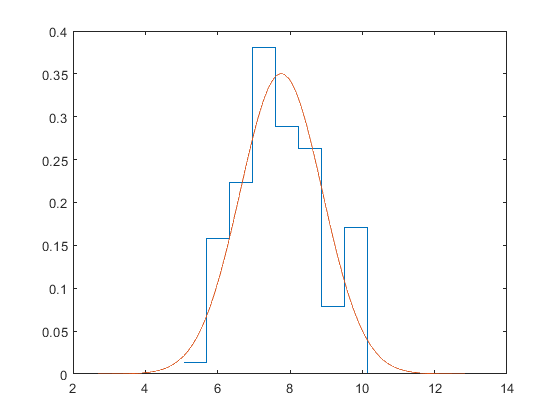
\includegraphics[scale=0.7]{img/1.png}
	\caption{Гистограмма и график функции плотности распределения вероятностей нормальной случайной величины с выборочными мат. ожиданием и дисперсией}
	\label{fig:1}
\end{figure}

\begin{figure}[H]
	\centering
	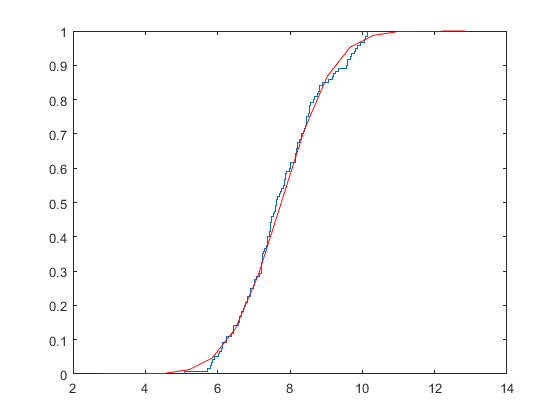
\includegraphics[scale=0.7]{img/2.png}
	\caption{График эмперической функции распределения и функции распределения нормальной случайной величины с выборочными мат. ожиданием и дисперсией}
	\label{fig:2}
\end{figure}

\bibliographystyle{utf8gost705u}  % стилевой файл для оформления по ГОСТу
\bibliography{51-biblio}          % имя библиографической базы (bib-файла)
	
\end{document}
